%
% welle.tex -- Bild zum Thema Optische Fouriertransformation <opt>
%
% (c) 2023 Marco Niederberger, Yanick Schoch; OST Ostschweizer Fachhochschule
%

\documentclass[tikz]{standalone}
% \usepackage{amsmath}
% \usepackage{txfonts}
% \usepackage{pgfplots}

% \pgfplotsset{compat=1.16}
\def\skala{1}

%
% opt_common.tex -- Commands and color definition for the paper <opt>
%
% (c) 2023 Marco Niederberger, Yanick Schoch; OST Ostschweizer Fachhochschule
%

%%% NEW COMMANDS %%%

% Lense (x, height, curvature)
\newcommand{\lense}[3]{
    \def\curvature{0.2}
    \path[fill=glass, draw=black, line width = 0.6, opacity=0.8] (#1,-#2) .. controls (#1 - #3,0) .. (#1,#2) .. controls (#1 + #3,0) .. (#1,-#2);
}

% Dimension arrow (xStart, xEnd, yHeight, text)
\newcommand{\optMeasurement}[4]{%
    \draw[<->] (#1, #3)--(#2, #3) node[above,midway] {#4};
}

% Annotated point
\newcommand{\point}[3]{
    \draw[fill=black] (#1) circle (1pt) node[#3] {#2};
}

%%% COLORS %%%

% Define Color
\definecolor{glass}{cmyk}{0.2,0,0,0}
\colorlet{optBlue}{blue!70!black}
\colorlet{optRed}{red!90!black}

%%% STYLES %%%

% Laser rays
\tikzset{red ray/.style = {optRed, line width = 0.6}}
\tikzset{ray arrow/.style = {red ray, postaction=decorate,decoration={markings,mark=at position 0.52 with \arrow{stealth}}}}


% \usetikzlibrary{arrows,intersections,math}
\usetikzlibrary{decorations.markings, } %calc


\begin{document}
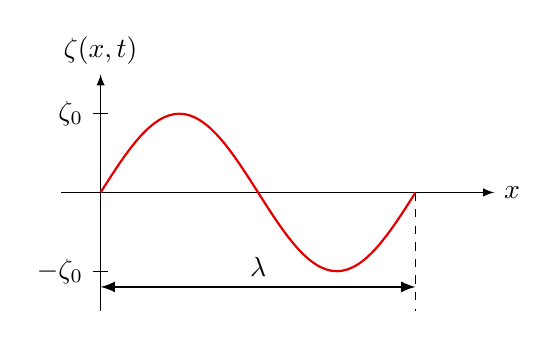
\begin{tikzpicture}[>=latex,thick,scale=\skala]
    % x and y axis
    \draw[->, thin] (-0.5,0)--(5,0) node[right]{$x$};
    \draw[->, thin] (0,-1.5)--(0,1.5) node[above]{$\zeta(x, t)$};
    \draw[-,thin] (-0.1,1)--(0.1,1) node[left=0.2cm]{$\zeta_0$};
    \draw[-,thin] (-0.1,-1)--(0.1,-1) node[left=0.2cm]{$-\zeta_0$};

    % Sine function
    \draw[optRed] (0,0) sin (1,1);
    \draw[optRed] (1,1) cos (2,0);
    \draw[optRed] (2,0) sin (3,-1);
    \draw[optRed] (3,-1) cos (4,0);

    % Measurement
    \optMeasurement{0}{4}{-1.2}{$\lambda$}
    \draw[-,thin, dashed] (4,0)--(4,-1.5);
\end{tikzpicture}
\end{document}

